\section{Supplementary information}
% * <emcowdery@gmail.com> 2018-04-12T07:10:44.396Z:
% 
% > Supplementary information
% Just a general note for the plots - I would avoid some of the really bright neon colors. I feel like they never print well and can make a figure hard to read (like for example figure 23) 
% 
% ^.

\begin{figure}
  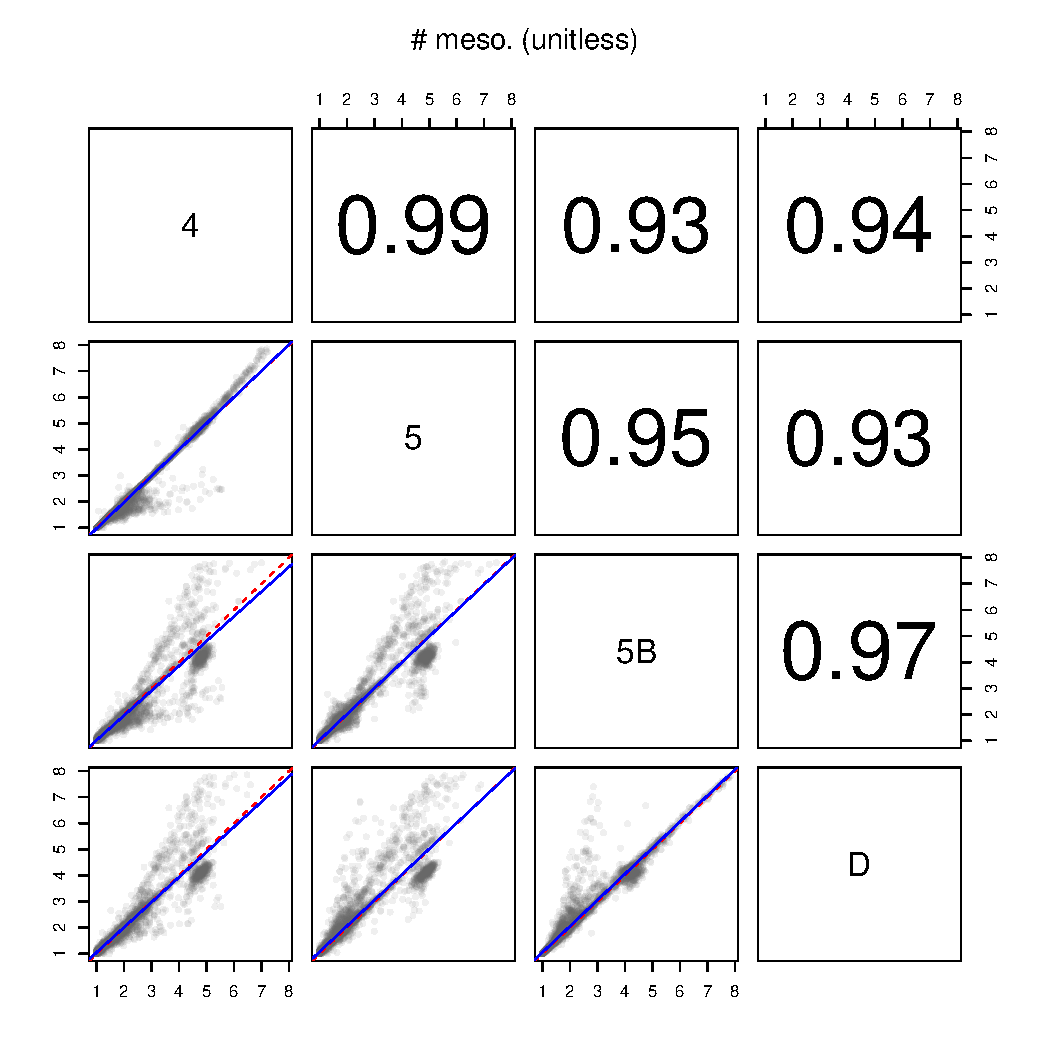
\includegraphics[width=\textwidth]{{figures/prospect_pairs_N}.png}
  \caption{\
    Inter-version comparison of estimates of number of leaf mesophyll structure.
  }\label{fig:prospect_pairs_N}
\end{figure}

\begin{figure}
  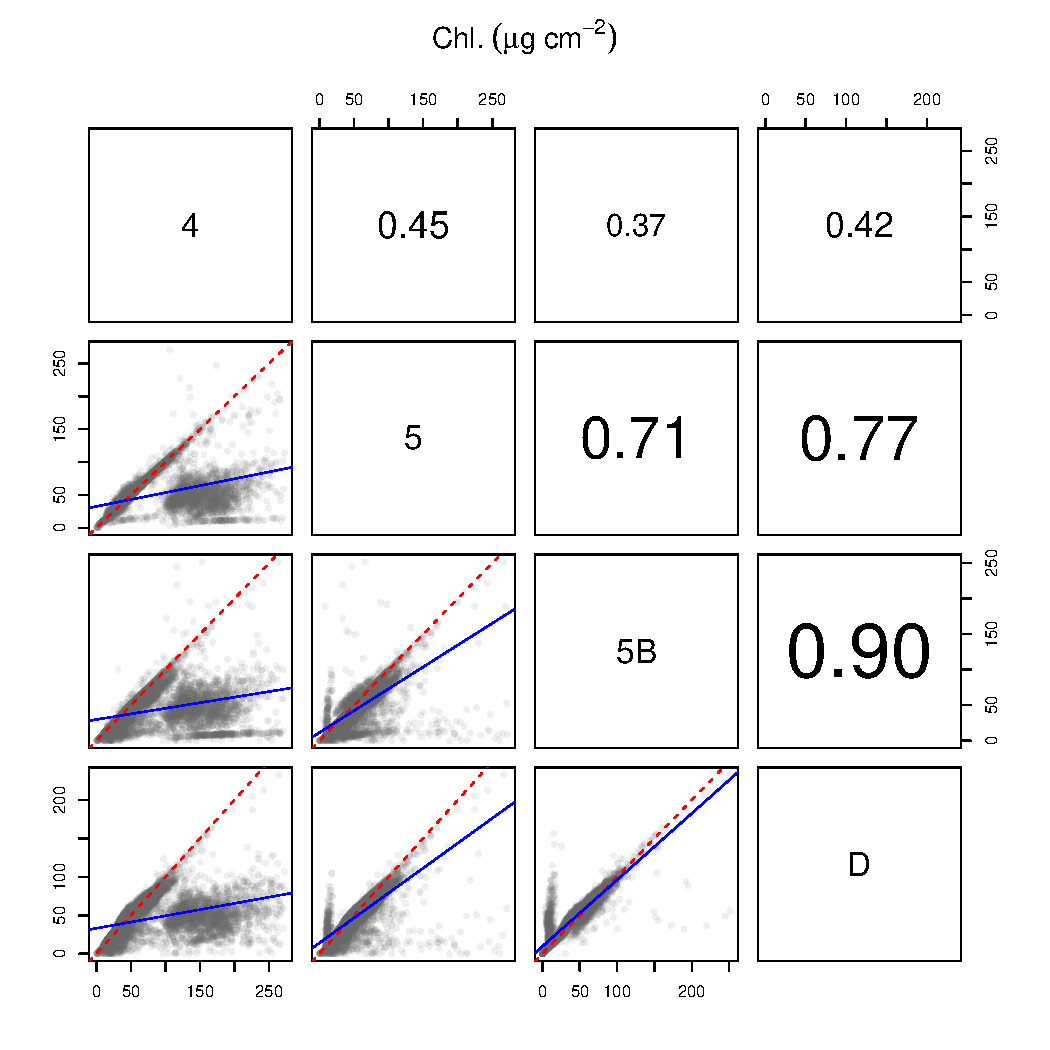
\includegraphics[width=\textwidth]{{figures/prospect_pairs_Cab}.png}
  \caption{\
    Inter-version comparison of estimates of number of total leaf chlorophyll content.
  }\label{fig:prospect_pairs_Cab}
\end{figure}

\begin{figure}
  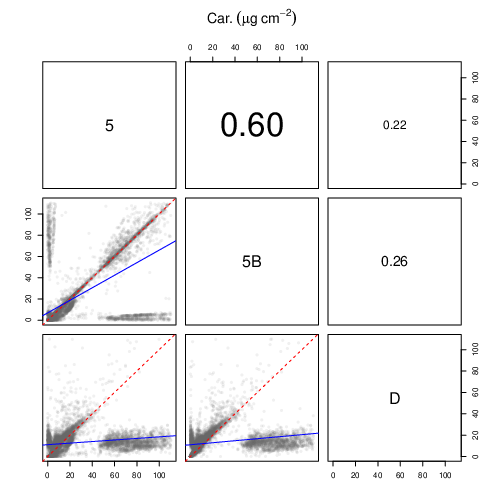
\includegraphics[width=\textwidth]{{figures/prospect_pairs_Car}.png}
  \caption{\
    Inter-version comparison of estimates of number of total leaf carotenoid content.
  }\label{fig:prospect_pairs_Car}
\end{figure}

\begin{figure}
  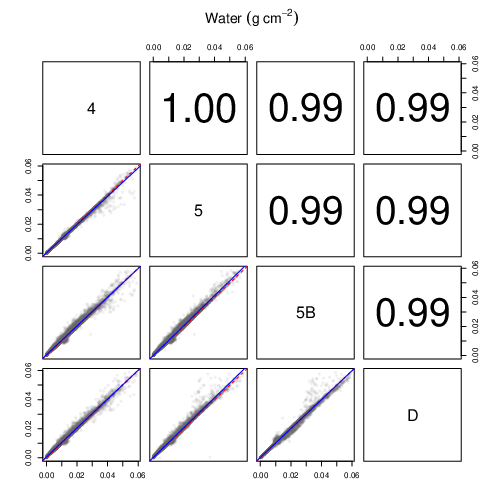
\includegraphics[width=\textwidth]{{figures/prospect_pairs_Cw}.png}
  \caption{\
    Inter-version comparison of estimates of number of total leaf water content.
  }\label{fig:prospect_pairs_Cw}
\end{figure}

\begin{figure}
  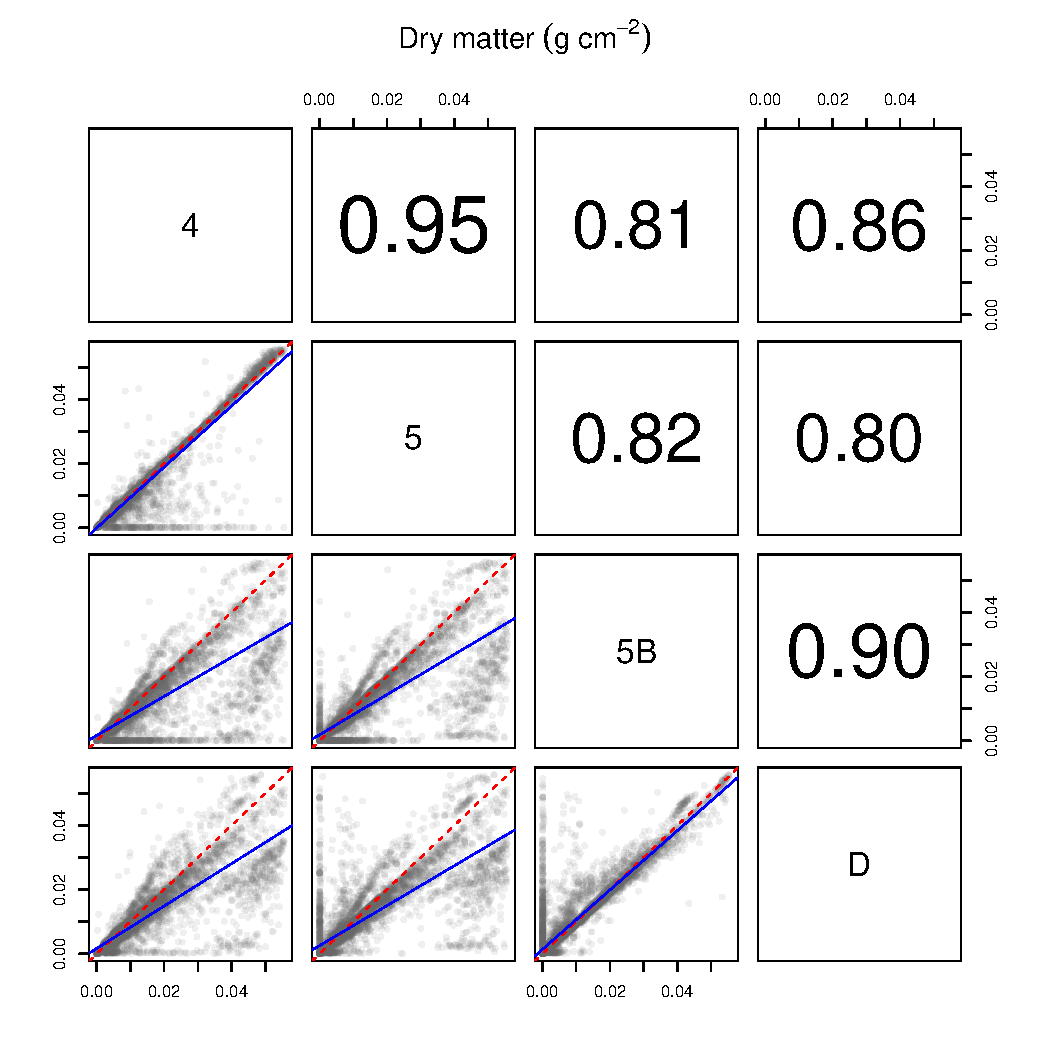
\includegraphics[width=\textwidth]{{figures/prospect_pairs_Cm}.png}
  \caption{\
    Inter-version comparison of estimates of number of total leaf dry matter content.
  }\label{fig:prospect_pairs_Cm}
\end{figure}

The extent of agreement on trait estimates between different versions of PROSPECT was strongly trait-dependent.
The most consistent inversion estimates were for leaf water content (Figure~\ref{fig:prospect_pairs_Cw}), which has a deep, wide-ranging, physically-based absorption coefficient that has not changed over the recent history of PROSPECT development~\cite{feret2008_prospect,feret2017_prospectd}.
Retrievals of the effective number of leaf mesophyll layers (Figure~\ref{fig:prospect_pairs_N}) and leaf dry matter content (Figure~\ref{fig:prospect_pairs_Cm}) were slightly less but still highly consistent across versions, despite changes in the refractive index and absorption features of the remaining PROSPECT parameters.
The ability of more recent versions of PROSPECT to differentiate between different types of pigments resulted in significant differences in pigment estimates between PROSPECT versions.
% * <dietze@bu.edu> 2018-04-11T13:08:00.421Z:
% 
% > The ability of more recent versions of PROSPECT to differentiate between different types of pigments resulted in significant differences in pigment estimates between PROSPECT versions.
% 
% This is important but buried -- for a lot of these you don't EXPECT the estimates to be the same and thus all of these figures paint a misleading picture. Also, there's a lot more of these figures than there really needs to be given that this doesn't seem to be like a central question -- feels like something that's mostly supplemental.
% 
% ^.
For chlorophyll content, the general trend is that the addition of additional pigments into the model (carotenoids in version 4, senescent brown pigments in 5, and anthocyanins in D) tends to reduce chlorophyll estimates, with the largest change happening between versions 4 and 5 (Figure~\ref{fig:prospect_pairs_Cab}).
The most significant across-version differences were in estimates of carotenoid concentrations, particularly between PROSPECT 5/5B and D, where the addition of anthocyanins led to significant reductions in estimates of carotenoid concentrations at the top of their range (Figure~\ref{fig:prospect_pairs_Car}).


\begin{figure}
  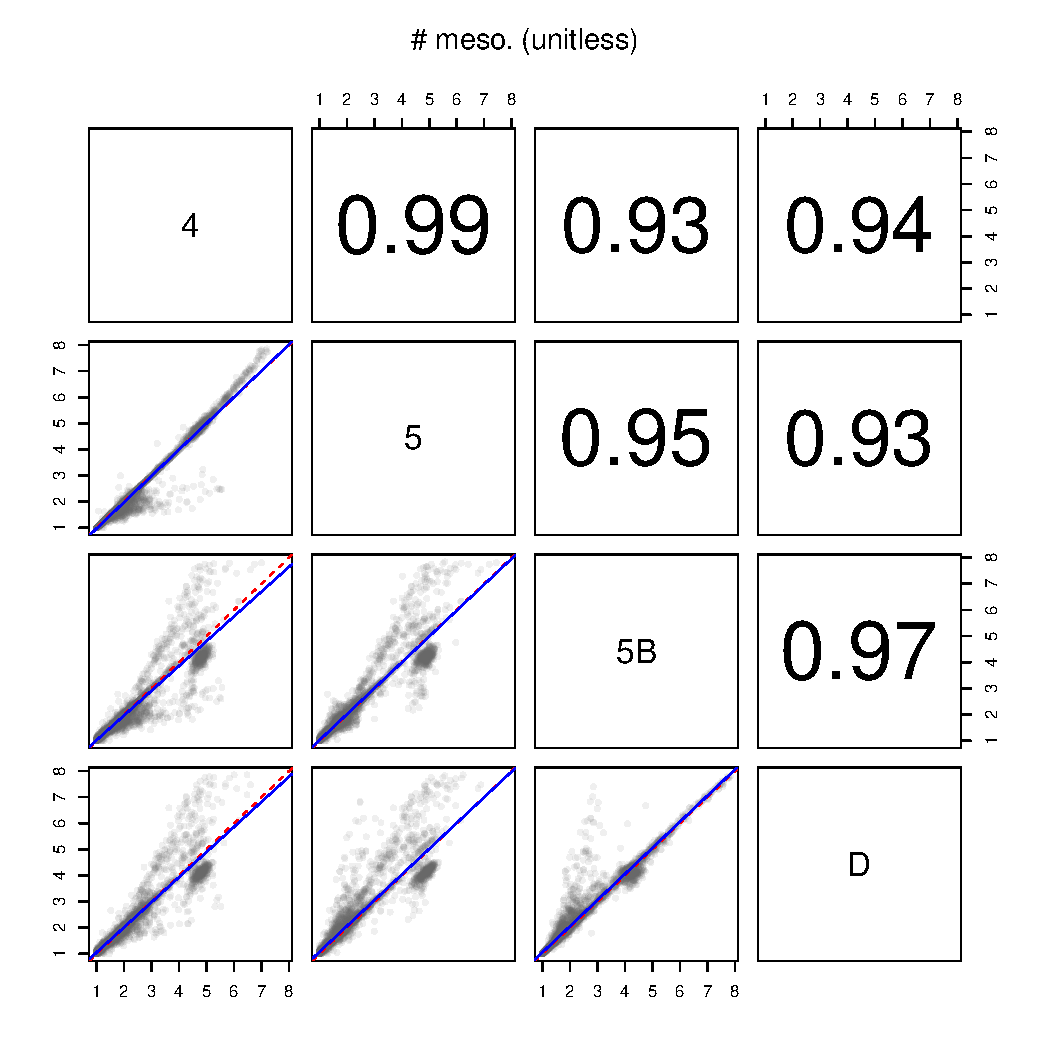
\includegraphics[width=\textwidth]{{figures/prospect_pairs_N}.png}
  \caption{\
    Inter-version comparison of estimates of number of leaf mesophyll structure.
  }\label{fig:prospect_pairs_N}
\end{figure}

\begin{figure}
  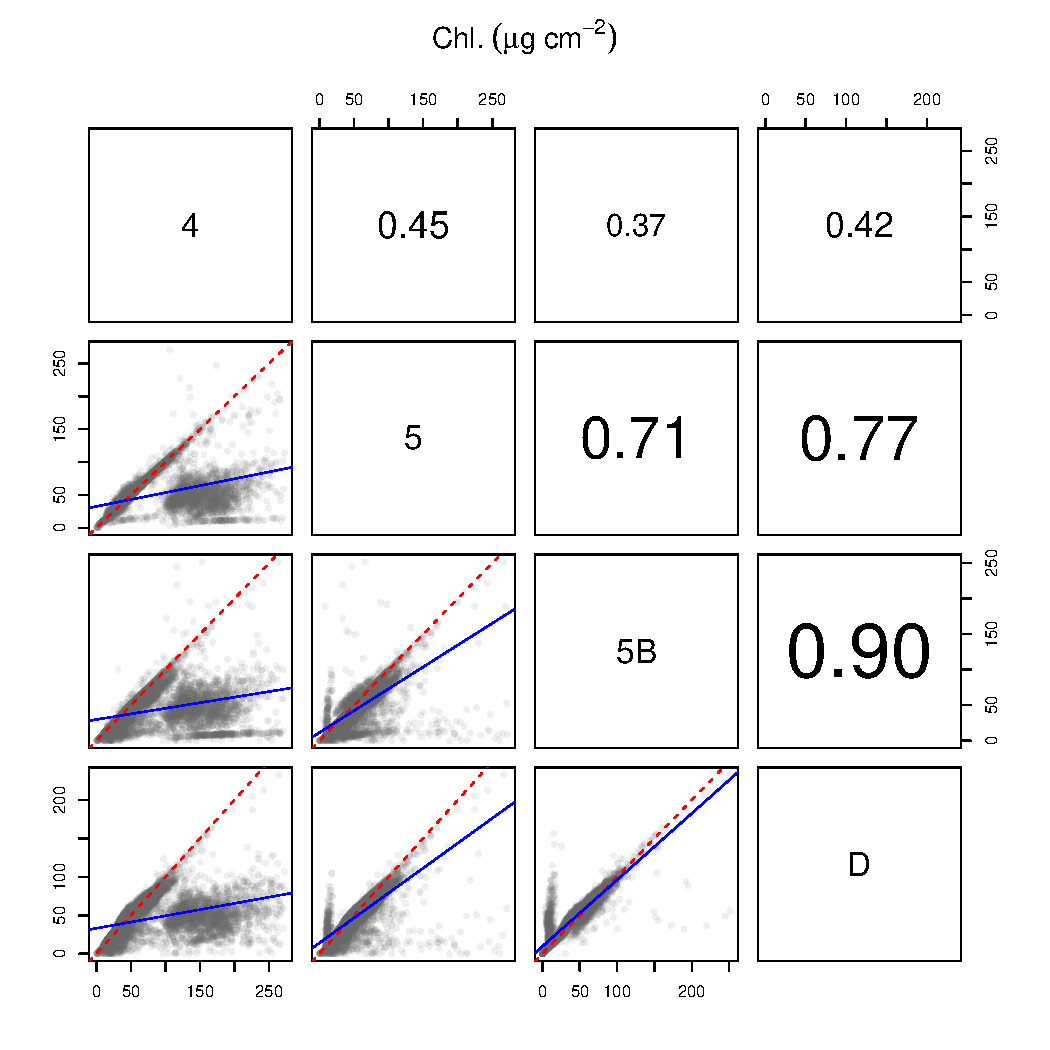
\includegraphics[width=\textwidth]{{figures/prospect_pairs_Cab}.png}
  \caption{\
    Inter-version comparison of estimates of number of total leaf chlorophyll content.
  }\label{fig:prospect_pairs_Cab}
\end{figure}

\begin{figure}
  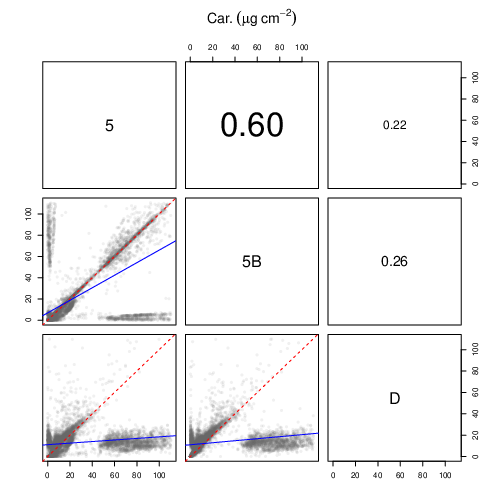
\includegraphics[width=\textwidth]{{figures/prospect_pairs_Car}.png}
  \caption{\
    Inter-version comparison of estimates of number of total leaf carotenoid content.
  }\label{fig:prospect_pairs_Car}
\end{figure}

\begin{figure}
  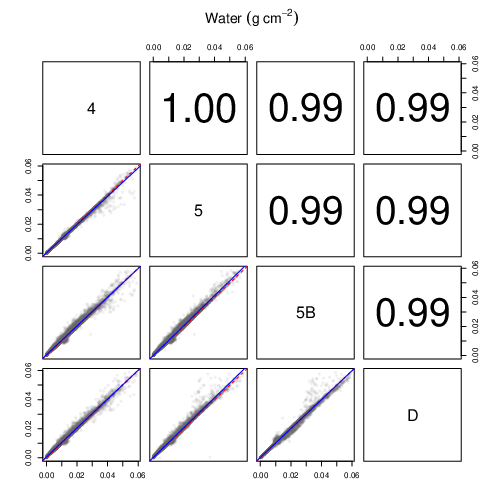
\includegraphics[width=\textwidth]{{figures/prospect_pairs_Cw}.png}
  \caption{\
    Inter-version comparison of estimates of number of total leaf water content.
  }\label{fig:prospect_pairs_Cw}
\end{figure}

\begin{figure}
  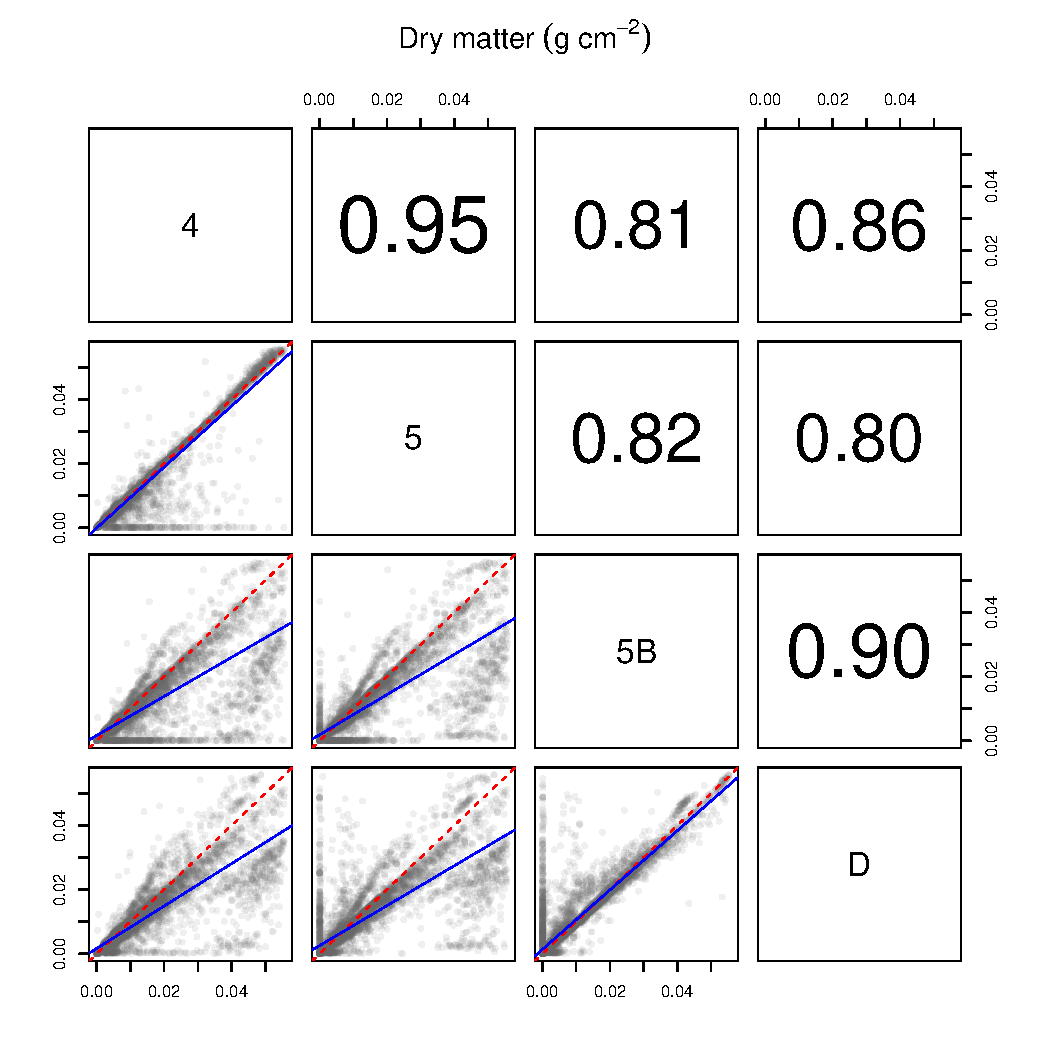
\includegraphics[width=\textwidth]{{figures/prospect_pairs_Cm}.png}
  \caption{\
    Inter-version comparison of estimates of number of total leaf dry matter content.
  }\label{fig:prospect_pairs_Cm}
\end{figure}

The extent of agreement on trait estimates between different versions of PROSPECT was strongly trait-dependent.
The most consistent inversion estimates were for leaf water content (Figure~\ref{fig:prospect_pairs_Cw}), which has a deep, wide-ranging, physically-based absorption coefficient that has not changed over the recent history of PROSPECT development~\cite{feret2008_prospect,feret2017_prospectd}.
Retrievals of the effective number of leaf mesophyll layers (Figure~\ref{fig:prospect_pairs_N}) and leaf dry matter content (Figure~\ref{fig:prospect_pairs_Cm}) were slightly less but still highly consistent across versions, despite changes in the refractive index and absorption features of the remaining PROSPECT parameters.
The ability of more recent versions of PROSPECT to differentiate between different types of pigments resulted in significant differences in pigment estimates between PROSPECT versions.
% * <dietze@bu.edu> 2018-04-11T13:08:00.421Z:
% 
% > The ability of more recent versions of PROSPECT to differentiate between different types of pigments resulted in significant differences in pigment estimates between PROSPECT versions.
% 
% This is important but buried -- for a lot of these you don't EXPECT the estimates to be the same and thus all of these figures paint a misleading picture. Also, there's a lot more of these figures than there really needs to be given that this doesn't seem to be like a central question -- feels like something that's mostly supplemental.
% 
% ^.
For chlorophyll content, the general trend is that the addition of additional pigments into the model (carotenoids in version 4, senescent brown pigments in 5, and anthocyanins in D) tends to reduce chlorophyll estimates, with the largest change happening between versions 4 and 5 (Figure~\ref{fig:prospect_pairs_Cab}).
The most significant across-version differences were in estimates of carotenoid concentrations, particularly between PROSPECT 5/5B and D, where the addition of anthocyanins led to significant reductions in estimates of carotenoid concentrations at the top of their range (Figure~\ref{fig:prospect_pairs_Car}).


\begin{figure}
  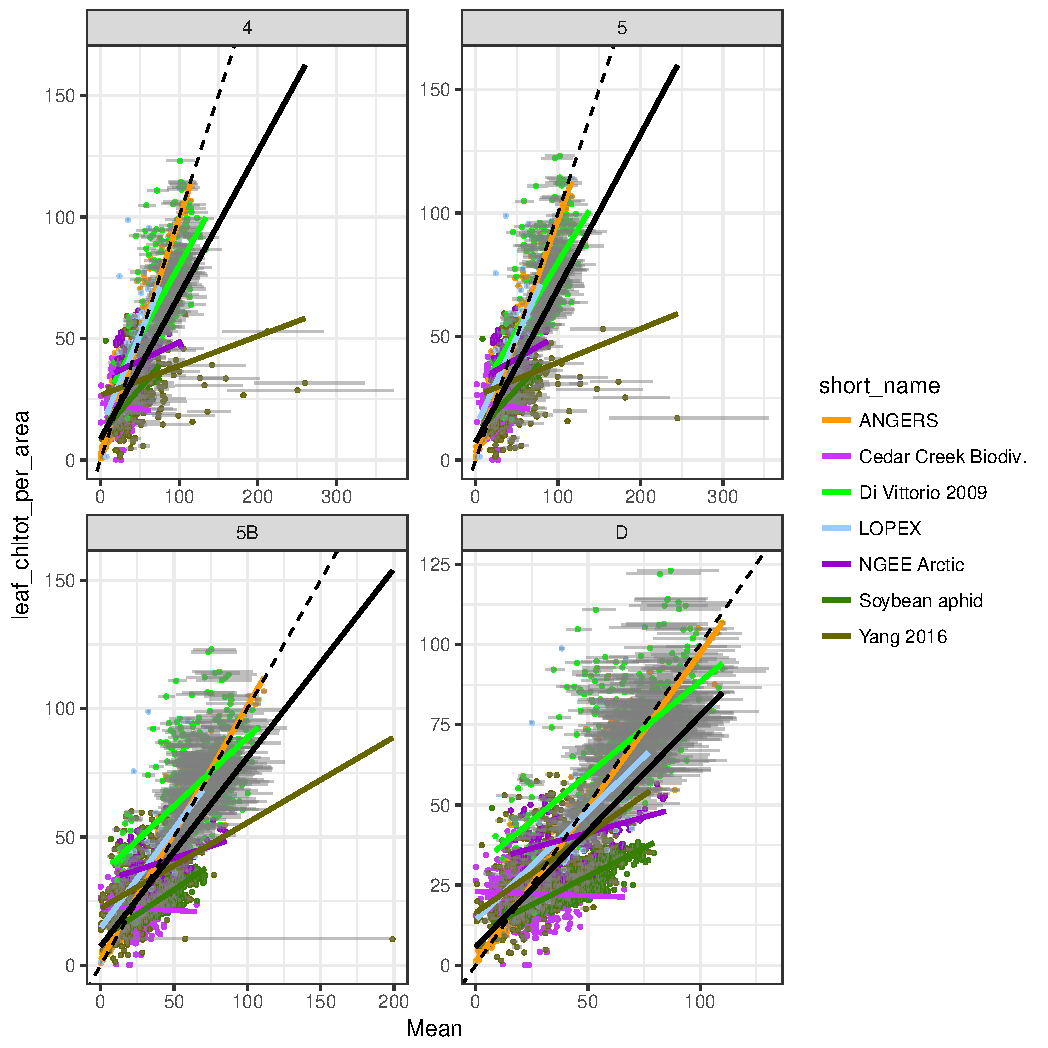
\includegraphics{{figures/validation_Cab}.pdf}
  \caption{Validation of leaf chlorophyll concentration}
  \label{fig:validation_cab}
\end{figure}

\begin{figure}
  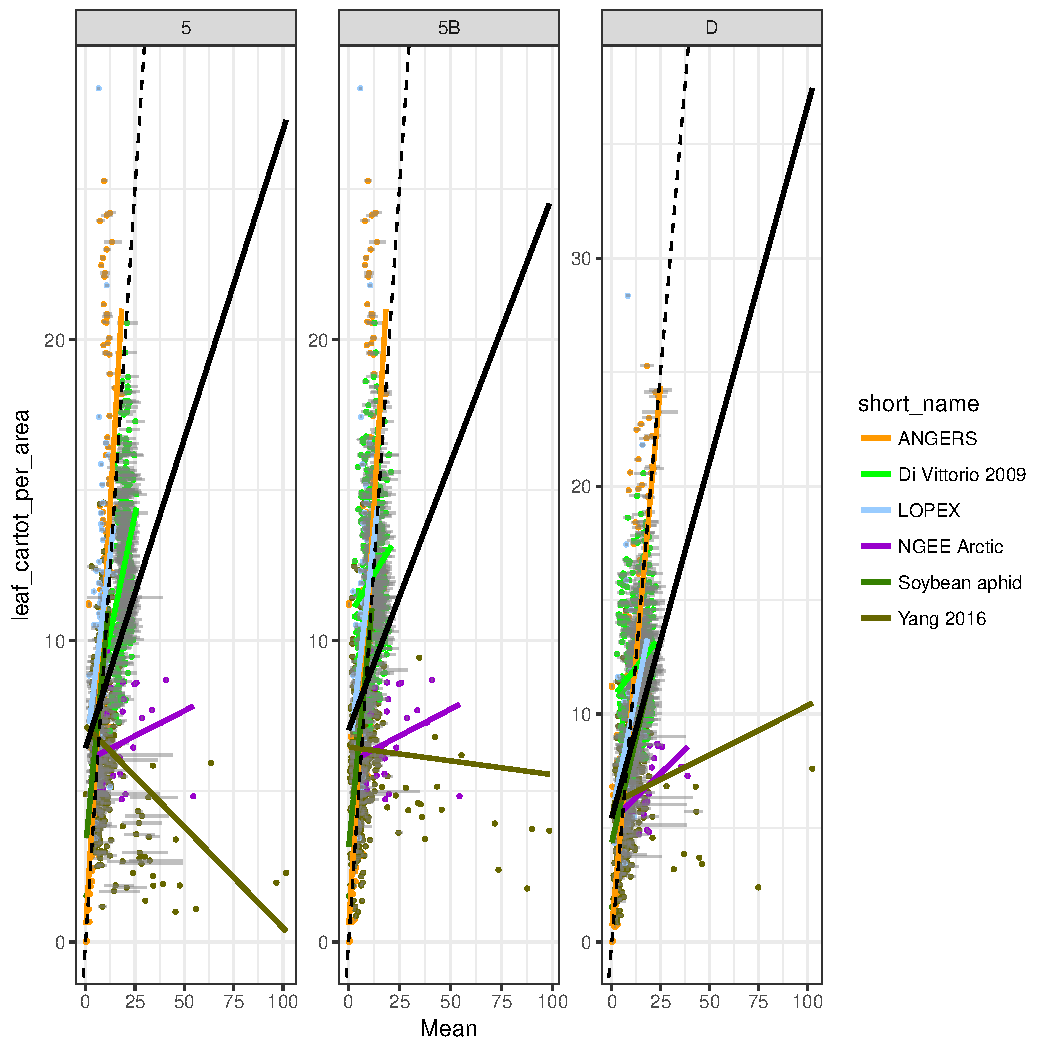
\includegraphics{{figures/validation_Car}.pdf}
  \caption{Validation of leaf carotenoid concentration}
  \label{fig:validation_car}
\end{figure}

\begin{figure}
  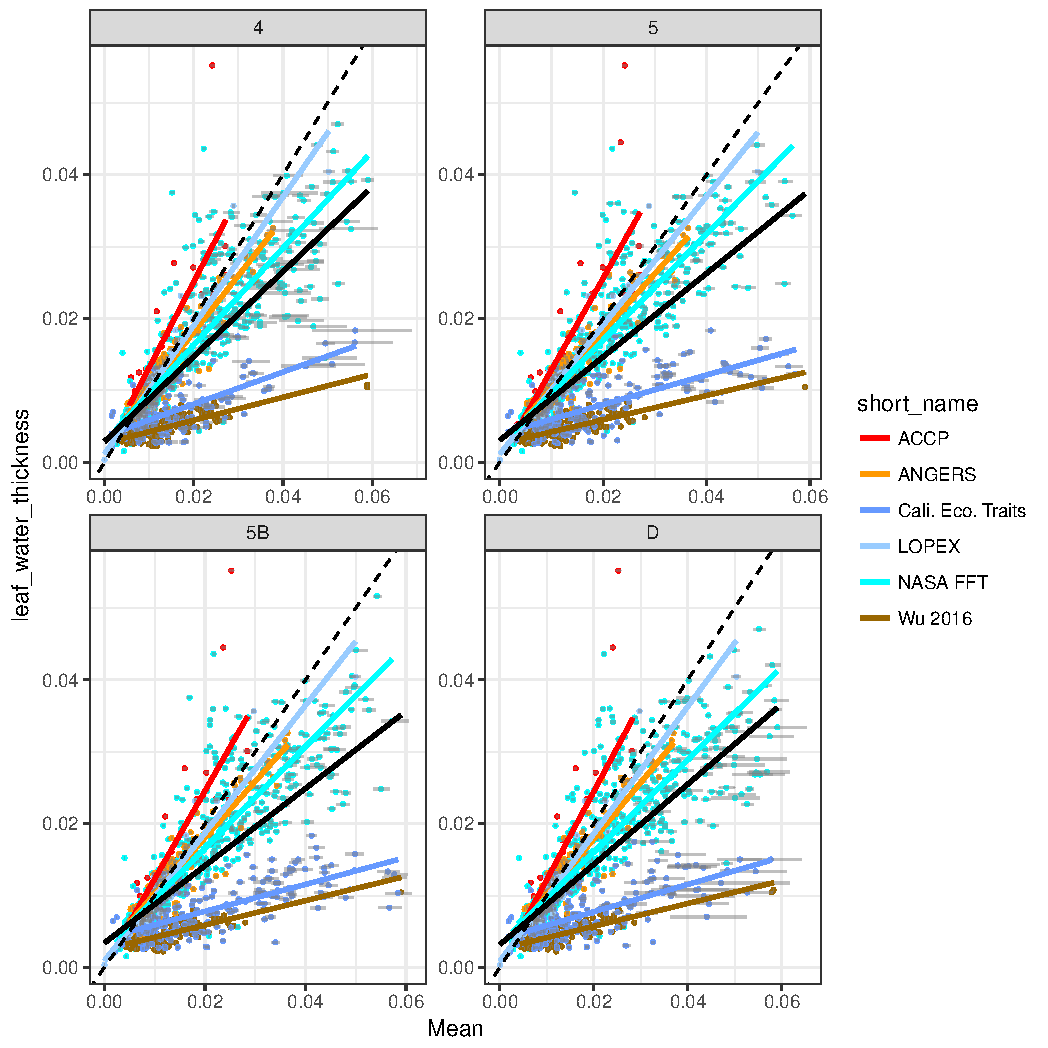
\includegraphics{{figures/validation_Cw}.pdf}
  \caption{Validation of leaf water content}
  \label{fig:validation_cw}
\end{figure}

\begin{figure}
  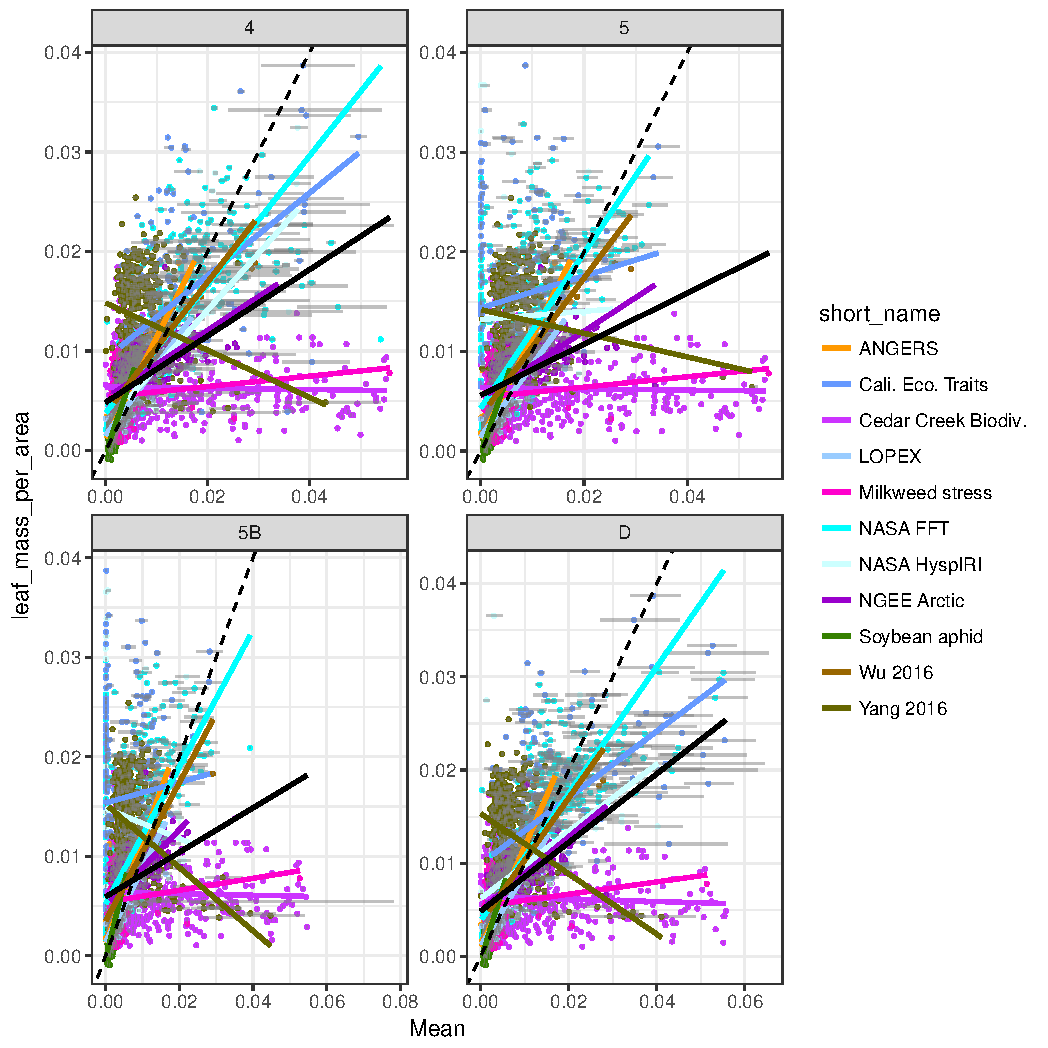
\includegraphics{{figures/validation_Cm}.pdf}
  \caption{Validation of leaf dry matter content}
  \label{fig:validation_cm}
\end{figure}

\begin{table}
  \caption{Inter-project comparison of PROSPECT validation for chlorophyll content}
  \begin{tabular}{llrrrr}
\toprule
Project & PROSPECT version & Slope & Intercept & R2 & MAE\\
\midrule
Cedar Creek Biodiv. & 5B & -0.0342156 & 23.063438 & 0.0021092 & 8.786800\\
Cedar Creek Biodiv. & 5 & -0.0415107 & 23.359903 & 0.0026898 & 7.762794\\
Cedar Creek Biodiv. & 4 & -0.0492768 & 23.505098 & 0.0035925 & 7.682664\\
Cedar Creek Biodiv. & D & -0.0256884 & 22.978977 & 0.0015396 & 8.993830\\
ANGERS & 5B & 0.9885100 & 2.029919 & 0.8943162 & 4.507075\\
\addlinespace
ANGERS & 5 & 0.9435222 & 2.848918 & 0.8927965 & 4.514387\\
ANGERS & 4 & 0.9690905 & 2.311719 & 0.8924498 & 4.575284\\
ANGERS & D & 0.9613827 & 1.071411 & 0.8940531 & 4.475625\\
Soybean aphid & 5B & 0.3841929 & 10.194932 & 0.7297580 & 12.680336\\
Soybean aphid & 5 & 0.3642454 & 10.561766 & 0.7590212 & 13.733716\\
\addlinespace
Soybean aphid & 4 & 0.3789026 & 10.510686 & 0.7497351 & 12.557874\\
Soybean aphid & D & 0.3564399 & 9.901860 & 0.7485083 & 16.215497\\
Yang 2016 & 5B & 0.3339415 & 22.128364 & 0.1921849 & 11.253180\\
Yang 2016 & 5 & 0.1358003 & 25.917848 & 0.0659116 & 18.050538\\
Yang 2016 & 4 & 0.1217998 & 26.601776 & 0.0712513 & 17.969556\\
\addlinespace
Yang 2016 & D & 0.4887395 & 16.411253 & 0.3311090 & 10.399497\\
Di Vittorio 2009 & 5B & 0.5335174 & 35.320336 & 0.3379697 & 13.433972\\
Di Vittorio 2009 & D & 0.5779908 & 30.586737 & 0.3986143 & 11.904135\\
Di Vittorio 2009 & 5 & 0.5537781 & 24.559954 & 0.4068840 & 18.171716\\
Di Vittorio 2009 & 4 & 0.5842066 & 21.478588 & 0.4634042 & 17.283023\\
\addlinespace
NGEE Arctic & 5B & 0.1849278 & 32.491348 & 0.1728367 & 13.025465\\
NGEE Arctic & 5 & 0.1891913 & 31.582062 & 0.1704651 & 13.467429\\
NGEE Arctic & 4 & 0.1536293 & 33.110428 & 0.1256801 & 14.496536\\
NGEE Arctic & D & 0.1939299 & 31.632261 & 0.1875215 & 13.896710\\
LOPEX & 5B & 0.7705550 & 14.508112 & 0.3708940 & 9.236673\\
\addlinespace
LOPEX & 5 & 0.7348981 & 13.219304 & 0.3946961 & 8.780386\\
LOPEX & 4 & 0.7722837 & 12.851069 & 0.3889503 & 8.806820\\
LOPEX & D & 0.6779585 & 14.121090 & 0.3620499 & 10.426814\\
\bottomrule
\end{tabular}
  \label{tab:r2_byproject_Cab}
\end{table}

\begin{table}
  \caption{Inter-project comparison of PROSPECT validation for carotenoid content}
  \begin{tabular}{llrrrr}
\toprule
Project & PROSPECT version & Slope & Intercept & R2 & MAE\\
\midrule
ANGERS & 5B & 1.1248574 & 0.4615427 & 0.5011801 & 2.308264\\
ANGERS & 5 & 1.1309651 & 0.3701458 & 0.4910904 & 2.296294\\
ANGERS & D & 0.9550749 & 0.6391524 & 0.7336856 & 1.566618\\
Soybean aphid & 5B & 0.6947568 & 3.1473650 & 0.8714765 & 1.209835\\
Soybean aphid & 5 & 0.6846229 & 3.1543269 & 0.8636690 & 1.134961\\
\addlinespace
Soybean aphid & D & 0.3689710 & 4.3788652 & 0.6927195 & 1.531178\\
Yang 2016 & 5B & -0.0091996 & 6.4733531 & 0.0014337 & 4.591324\\
Yang 2016 & 5 & -0.0671401 & 7.1771164 & 0.0654946 & 5.023418\\
Yang 2016 & D & 0.0430874 & 6.0525547 & 0.0180631 & 3.900997\\
Di Vittorio 2009 & 5B & 0.1119673 & 10.8122194 & 0.0260585 & 3.332397\\
\addlinespace
Di Vittorio 2009 & D & 0.1100432 & 10.6763771 & 0.0375479 & 3.895357\\
Di Vittorio 2009 & 5 & 0.3130490 & 6.3629754 & 0.1259879 & 6.871812\\
NGEE Arctic & 5B & 0.0356118 & 5.9541017 & 0.0858288 & 10.296848\\
NGEE Arctic & 5 & 0.0334094 & 6.0053053 & 0.0750289 & 10.656218\\
NGEE Arctic & D & 0.0834834 & 5.3134268 & 0.2775419 & 8.149149\\
\addlinespace
LOPEX & 5B & 0.5927136 & 6.0413940 & 0.1025811 & 3.622300\\
LOPEX & 5 & 0.5362923 & 6.2178865 & 0.0783836 & 3.520730\\
LOPEX & D & 0.4237720 & 5.5949372 & 0.1232201 & 3.235404\\
\bottomrule
\end{tabular}
  \label{tab:r2_byproject_Car}
\end{table}

\begin{table}
  \caption{Inter-project comparison of PROSPECT validation for water content}
  
\begin{tabular}{llrrrr}
\toprule
Project & PROSPECT version & Slope & Intercept & R2 & MAE\\
\midrule
ACCP & 5B & 1.2224154 & 0.0000975 & 0.6338263 & 0.0040751\\
ACCP & 5 & 1.2743726 & 0.0001449 & 0.6322688 & 0.0045025\\
ACCP & 4 & 1.1924129 & 0.0012373 & 0.5876346 & 0.0043745\\
ACCP & D & 1.2258934 & -0.0000465 & 0.6349863 & 0.0040316\\
NASA FFT & 5B & 0.7066325 & 0.0024628 & 0.8300954 & 0.0030940\\
\addlinespace
NASA FFT & 5 & 0.7369678 & 0.0022872 & 0.8343479 & 0.0027610\\
NASA FFT & 4 & 0.6743618 & 0.0028092 & 0.8040672 & 0.0032115\\
NASA FFT & D & 0.6435333 & 0.0031754 & 0.8046589 & 0.0037844\\
Wu 2016 & 5B & 0.1697077 & 0.0025033 & 0.5801156 & 0.0083944\\
Wu 2016 & 5 & 0.1684053 & 0.0025574 & 0.5699220 & 0.0083499\\
\addlinespace
Wu 2016 & 4 & 0.1596479 & 0.0026570 & 0.6049022 & 0.0085609\\
Wu 2016 & D & 0.1585126 & 0.0025586 & 0.6477039 & 0.0089523\\
ANGERS & 5B & 0.7837878 & 0.0023605 & 0.8724714 & 0.0012784\\
ANGERS & 5 & 0.8000370 & 0.0022369 & 0.8715782 & 0.0012390\\
ANGERS & 4 & 0.7867793 & 0.0023566 & 0.8735681 & 0.0012677\\
\addlinespace
ANGERS & D & 0.7853827 & 0.0021684 & 0.8734074 & 0.0012848\\
Cali. Eco. Traits & 5B & 0.1874567 & 0.0040570 & 0.4570087 & 0.0129114\\
Cali. Eco. Traits & 5 & 0.2055733 & 0.0039261 & 0.4867141 & 0.0111009\\
Cali. Eco. Traits & 4 & 0.2226823 & 0.0036425 & 0.4723009 & 0.0094627\\
Cali. Eco. Traits & D & 0.1900469 & 0.0039453 & 0.4206440 & 0.0112379\\
\addlinespace
LOPEX & 5B & 0.8886147 & 0.0009194 & 0.9208119 & 0.0013648\\
LOPEX & 5 & 0.8963794 & 0.0011431 & 0.9105920 & 0.0013501\\
LOPEX & 4 & 0.8936068 & 0.0011562 & 0.9118809 & 0.0013394\\
LOPEX & D & 0.8854889 & 0.0008703 & 0.9186307 & 0.0013871\\
\bottomrule
\end{tabular}
  \label{tab:r2_byproject_Cw}
\end{table}

\begin{table}
  \caption{Inter-project comparison of PROSPECT validation for dry matter content}
  \begin{tabular}{llrrrr}
\toprule
Project & PROSPECT version & Slope & Intercept & R2 & MAE\\
\midrule
Cedar Creek Biodiv. & 5B & -0.0072848 & 0.0063759 & 0.0008256 & 0.0072626\\
Cedar Creek Biodiv. & 5 & -0.0060881 & 0.0063616 & 0.0006306 & 0.0075502\\
Cedar Creek Biodiv. & 4 & -0.0065251 & 0.0063956 & 0.0007300 & 0.0076035\\
Cedar Creek Biodiv. & D & -0.0131477 & 0.0064098 & 0.0027579 & 0.0072127\\
NASA FFT & 5B & 0.6877940 & 0.0052184 & 0.3379753 & 0.0038709\\
\addlinespace
NASA FFT & 5 & 0.7785810 & 0.0042846 & 0.4665472 & 0.0034032\\
NASA FFT & 4 & 0.6460322 & 0.0037878 & 0.6966649 & 0.0027552\\
NASA FFT & D & 0.6812059 & 0.0038455 & 0.7612321 & 0.0027699\\
NASA HyspIRI & 5B & -0.1523223 & 0.0148298 & 0.0130478 & 0.0095169\\
NASA HyspIRI & 5 & 0.0412560 & 0.0132023 & 0.0008450 & 0.0074109\\
\addlinespace
NASA HyspIRI & 4 & 0.5711822 & 0.0026934 & 0.5765417 & 0.0052037\\
NASA HyspIRI & D & 0.3609614 & 0.0061894 & 0.2459108 & 0.0052854\\
Wu 2016 & 5B & 0.6952496 & 0.0034879 & 0.7711302 & 0.0018656\\
Wu 2016 & 5 & 0.6916600 & 0.0035188 & 0.7753852 & 0.0018793\\
Wu 2016 & 4 & 0.6605134 & 0.0037330 & 0.7833351 & 0.0019289\\
\addlinespace
Wu 2016 & D & 0.6677423 & 0.0036331 & 0.7590705 & 0.0018922\\
ANGERS & 5B & 1.0281975 & 0.0012374 & 0.7381387 & 0.0014149\\
ANGERS & 5 & 1.0344467 & 0.0011414 & 0.7988216 & 0.0013502\\
ANGERS & 4 & 1.0330004 & 0.0010591 & 0.8117388 & 0.0013044\\
ANGERS & D & 1.0898614 & 0.0008806 & 0.7849743 & 0.0013056\\
\addlinespace
Cali. Eco. Traits & 5B & 0.1036178 & 0.0153586 & 0.0053226 & 0.0105736\\
Cali. Eco. Traits & 5 & 0.1606825 & 0.0143608 & 0.0172288 & 0.0093219\\
Cali. Eco. Traits & 4 & 0.4169109 & 0.0092271 & 0.2684472 & 0.0063485\\
Cali. Eco. Traits & D & 0.3556755 & 0.0099264 & 0.3224713 & 0.0068044\\
Soybean aphid & 5B & 1.4998023 & -0.0002306 & 0.6850881 & 0.0010973\\
\addlinespace
Soybean aphid & 5 & 1.4992713 & -0.0002585 & 0.7053147 & 0.0010790\\
Soybean aphid & 4 & 1.5078288 & -0.0002826 & 0.7043454 & 0.0010809\\
Soybean aphid & D & 1.5432541 & -0.0004485 & 0.6841007 & 0.0010669\\
Milkweed stress & 5B & 0.0600668 & 0.0053841 & 0.0043586 & 0.0029551\\
Milkweed stress & 5 & 0.0520910 & 0.0053754 & 0.0037562 & 0.0028633\\
\addlinespace
Milkweed stress & 4 & 0.0523803 & 0.0053897 & 0.0038057 & 0.0028759\\
Milkweed stress & D & 0.0660527 & 0.0053479 & 0.0049127 & 0.0028890\\
Yang 2016 & 5B & -0.3182721 & 0.0152240 & 0.1342862 & 0.0079426\\
Yang 2016 & 5 & -0.1188457 & 0.0142006 & 0.0151085 & 0.0073769\\
Yang 2016 & 4 & -0.2375932 & 0.0148436 & 0.0483478 & 0.0074810\\
\addlinespace
Yang 2016 & D & -0.3236613 & 0.0153245 & 0.1098288 & 0.0078003\\
NGEE Arctic & 5B & 0.3836777 & 0.0049987 & 0.6162531 & 0.0022636\\
NGEE Arctic & 5 & 0.3387946 & 0.0052446 & 0.5560421 & 0.0023420\\
NGEE Arctic & 4 & 0.3407793 & 0.0052566 & 0.5598917 & 0.0023529\\
NGEE Arctic & D & 0.3902815 & 0.0050045 & 0.5805432 & 0.0021664\\
\addlinespace
LOPEX & 5B & 0.7449896 & 0.0013263 & 0.7126398 & 0.0008655\\
LOPEX & 5 & 0.7230686 & 0.0014063 & 0.6921972 & 0.0009416\\
LOPEX & 4 & 0.7041537 & 0.0015084 & 0.6834279 & 0.0009598\\
LOPEX & D & 0.7825339 & 0.0010571 & 0.7297655 & 0.0008504\\
\bottomrule
\end{tabular}
  \label{tab:r2_byproject_Cm}
\end{table}

\begin{figure}
  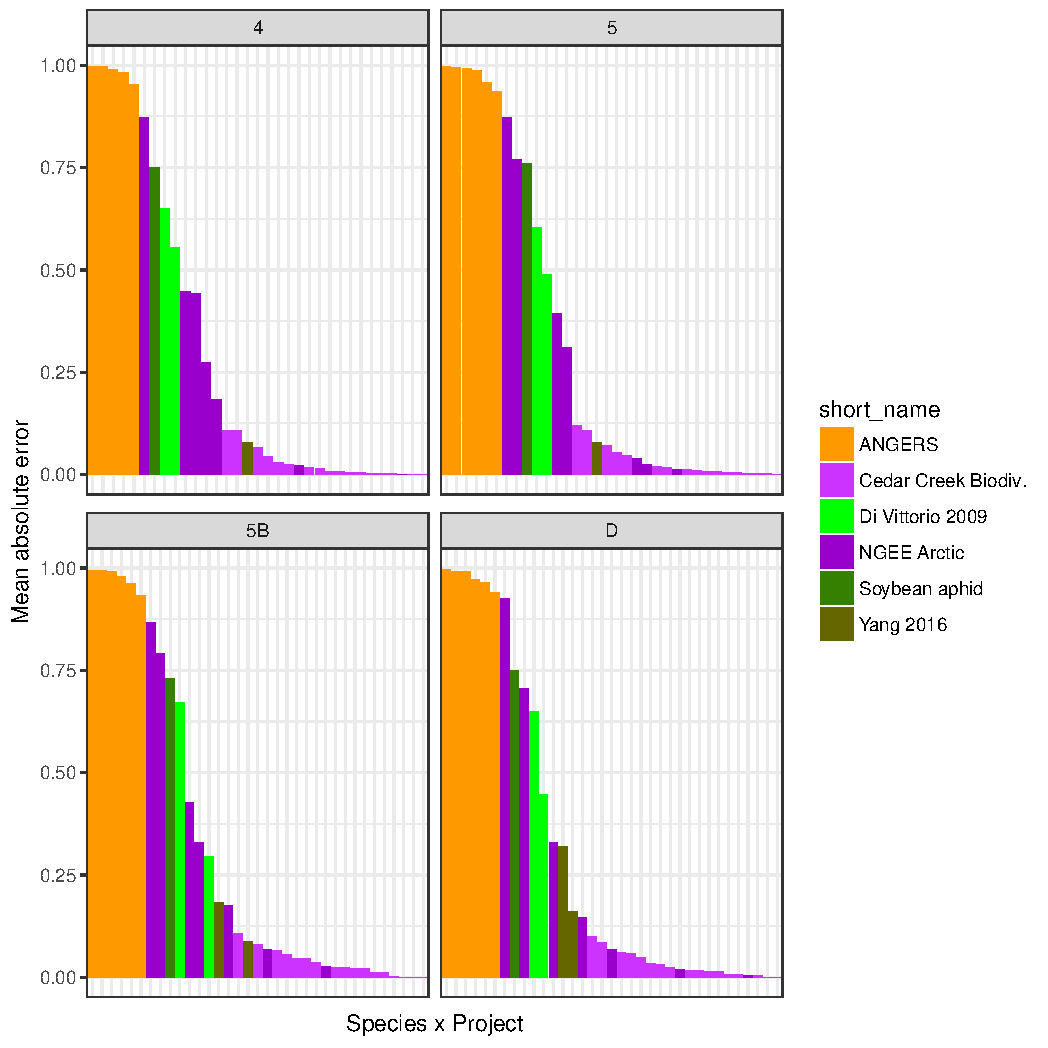
\includegraphics{{figures/r2_speciesbyproj_Cab}.pdf}
  \caption{Mean absolute error in PROSPECT inversion by species and project for chlorophyll content}
  \label{fig:error_speciesbyproj_Cab}
\end{figure}

\begin{figure}
  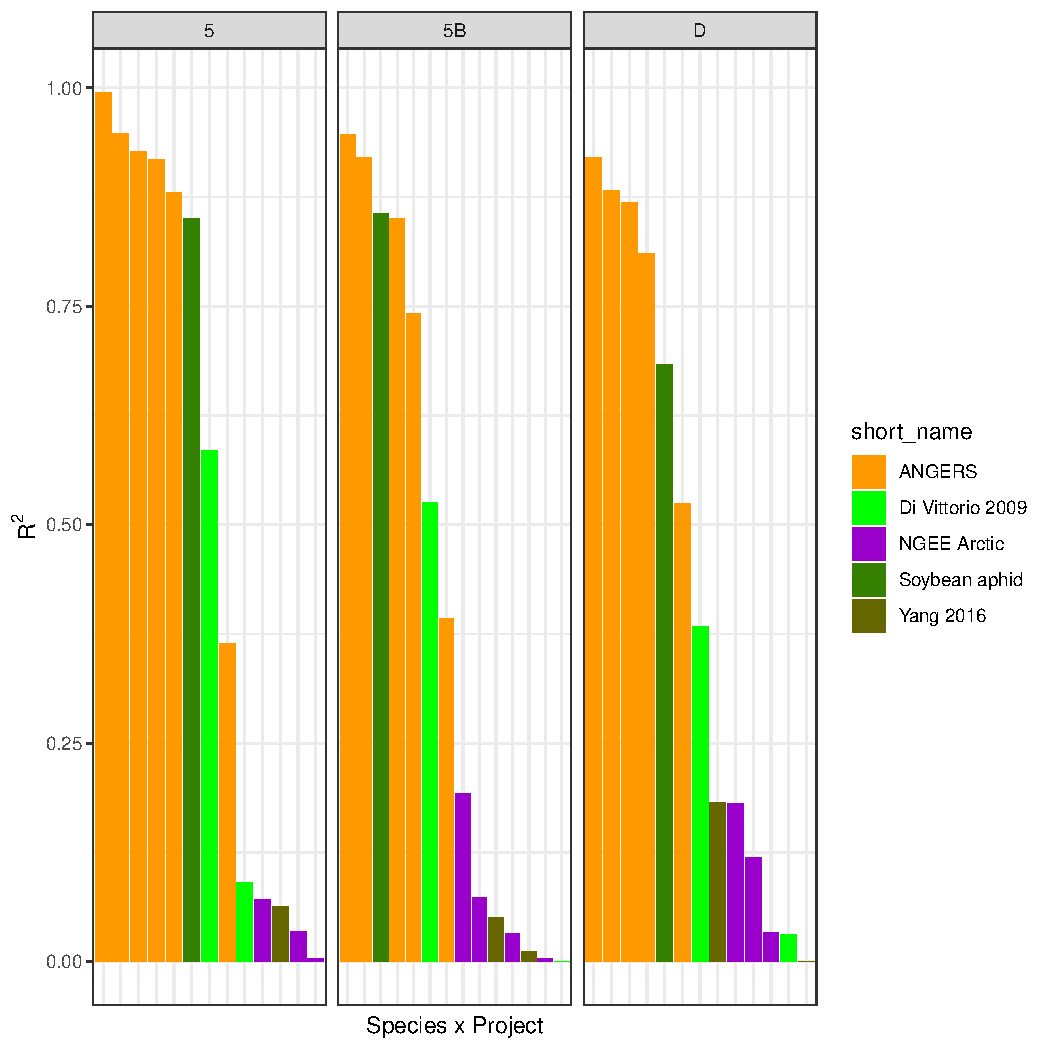
\includegraphics{{figures/r2_speciesbyproj_Car}.pdf}
  \caption{Mean absolute error in PROSPECT inversion by species and project for carotenoid content}
  \label{fig:error_speciesbyproj_Car}
\end{figure}

\begin{figure}
  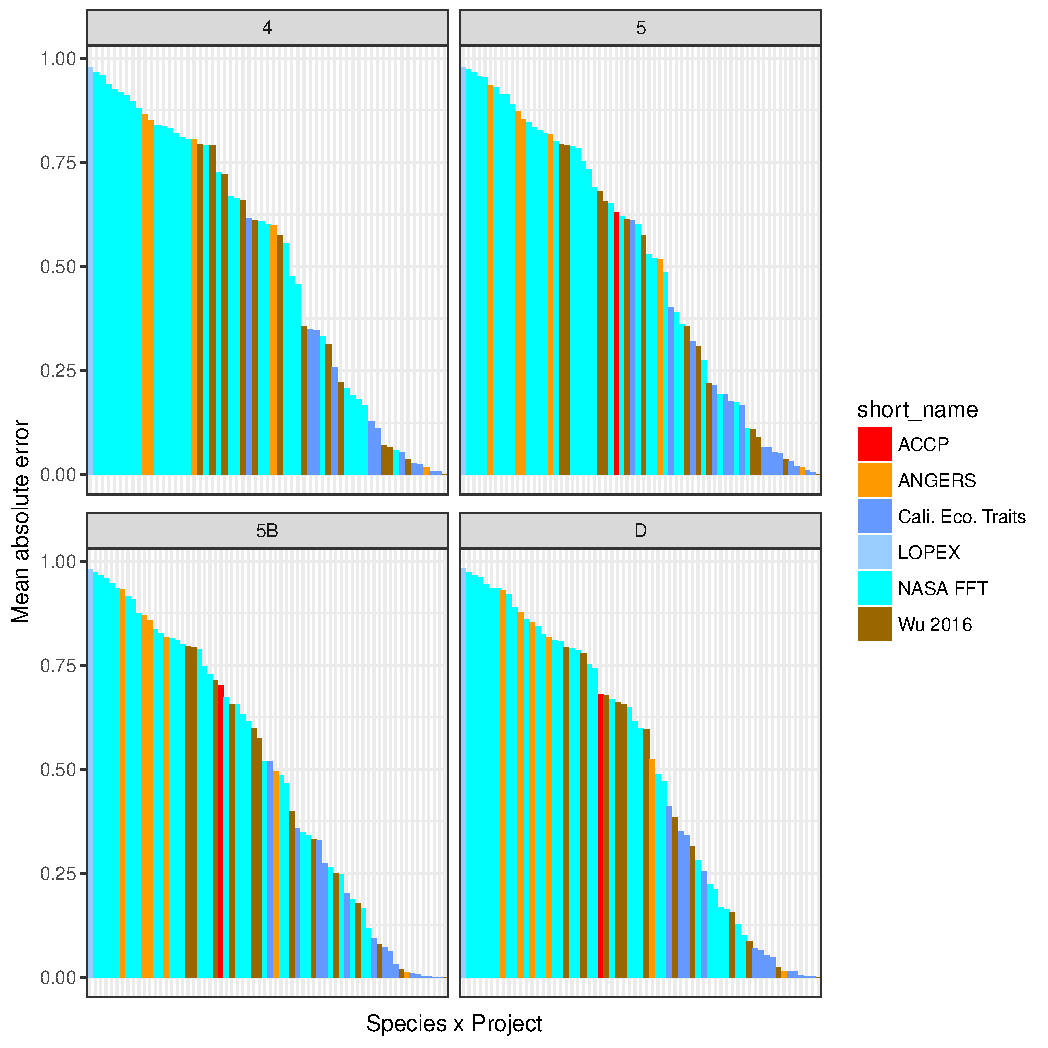
\includegraphics{{figures/r2_speciesbyproj_Cw}.pdf}
  \caption{Mean absolute error in PROSPECT inversion by species and project for leaf water content}
  \label{fig:error_speciesbyproj_Cw}
\end{figure}

\begin{figure}
  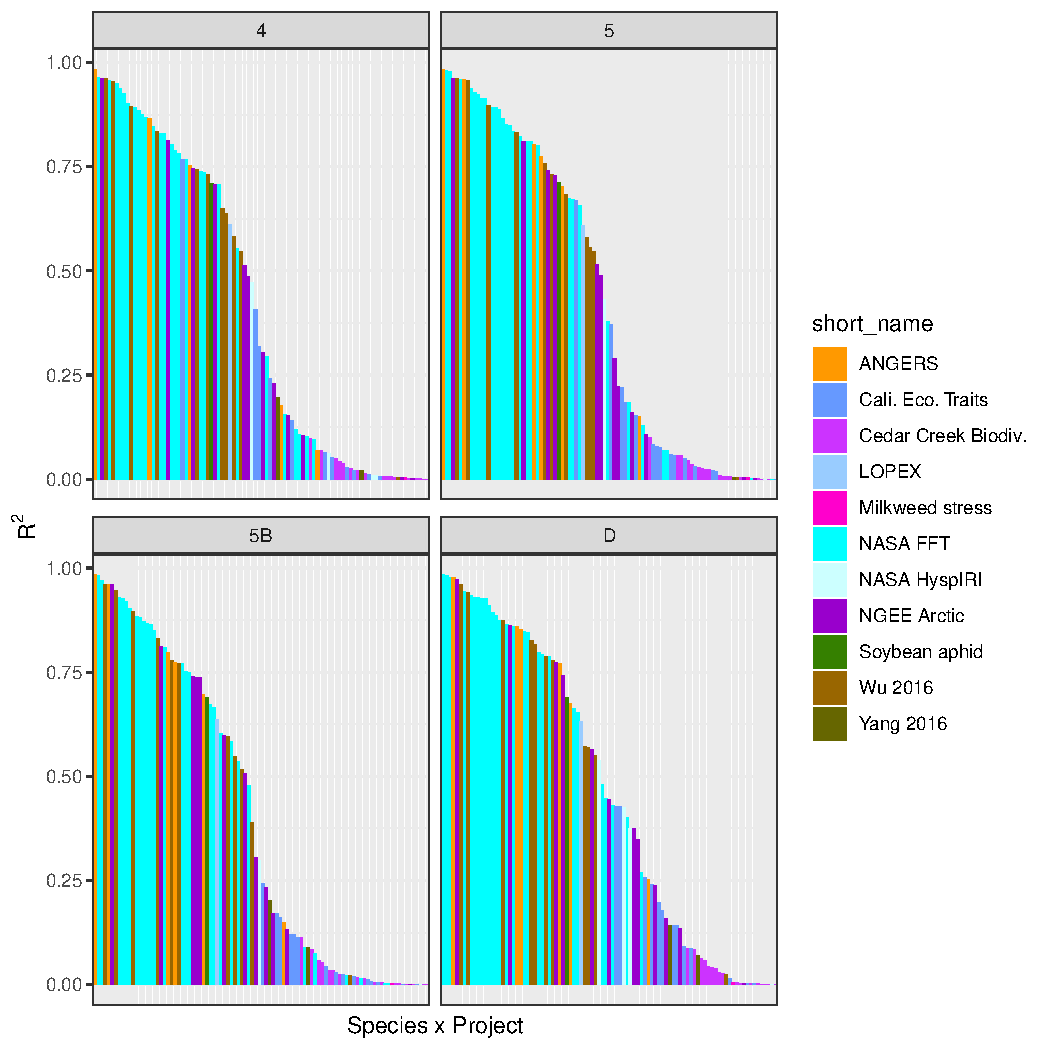
\includegraphics{{figures/r2_speciesbyproj_Cm}.pdf}
  \caption{Mean absolute error in PROSPECT inversion by species and project for leaf dry matter content}
  \label{fig:error_speciesbyproj_Cm}
\end{figure}

\begin{figure}
  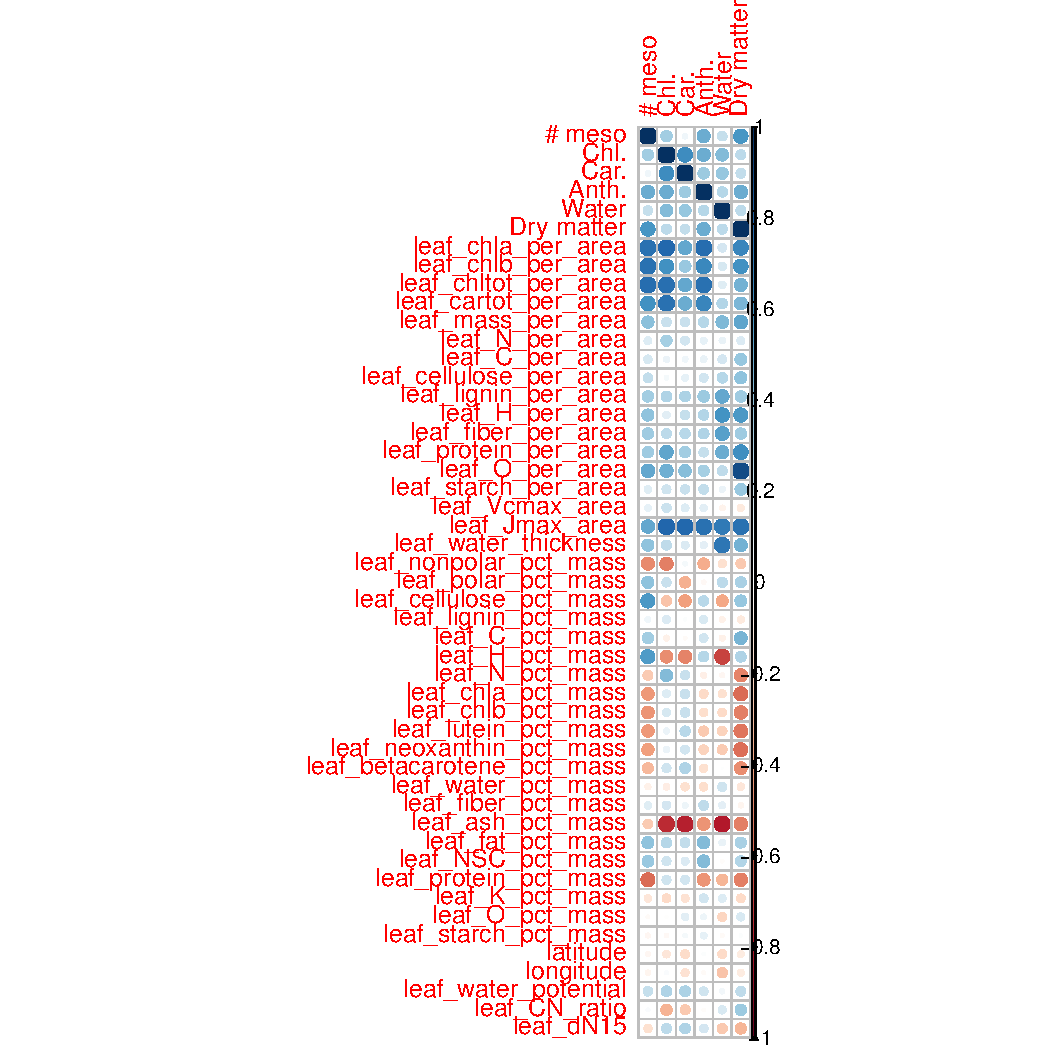
\includegraphics[width=\textwidth]{{figures/trait_correlations_all}.pdf}
  \caption{\
    Correlations of optical trait estimates with direct trait measurements, by all observations.
  }\label{fig:trait_correlations_all}
\end{figure}

\begin{figure}
  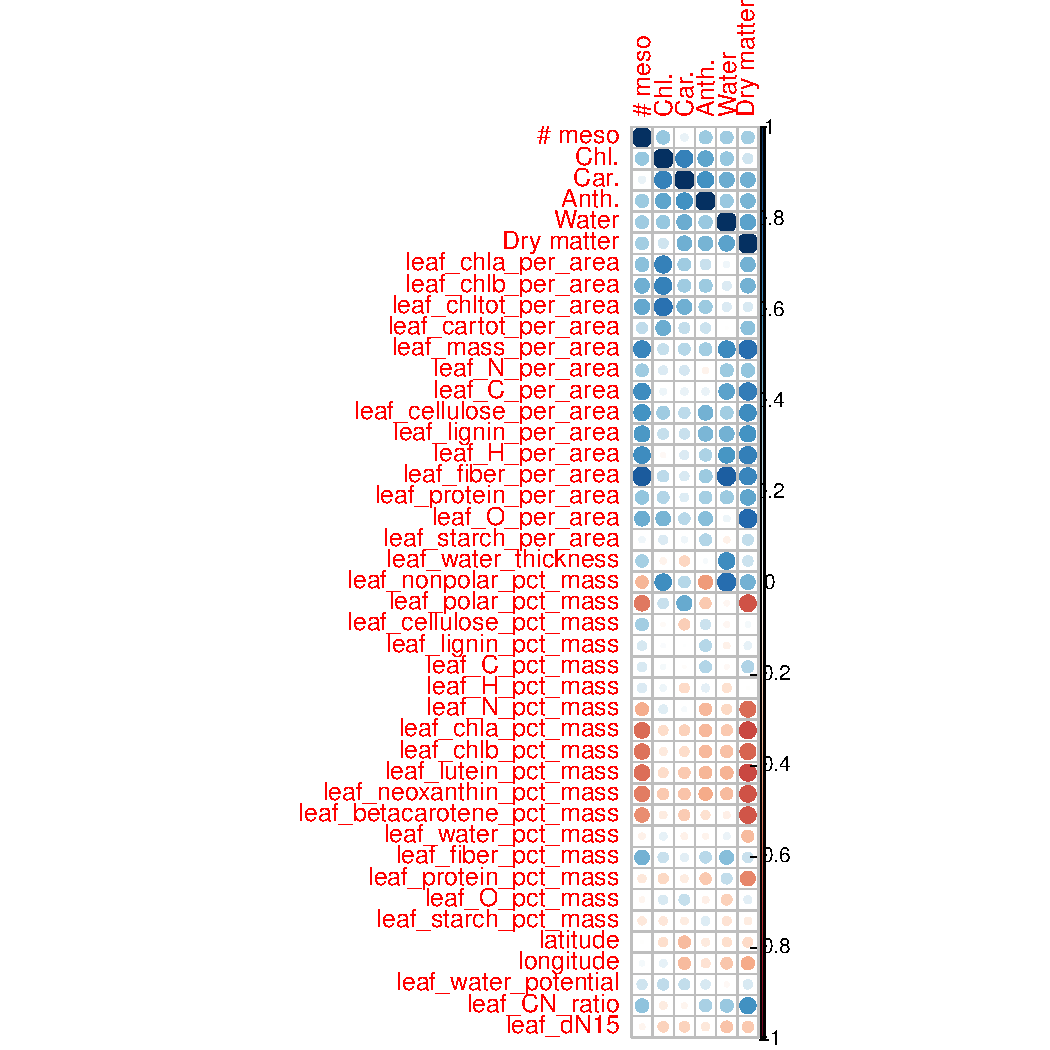
\includegraphics[width=\textwidth]{{figures/trait_correlations_species}.pdf}
  \caption{\
    Correlations of optical trait estimates with direct trait measurements, by species means.
  }\label{fig:trait_correlations_species}
\end{figure}

